\documentclass[10pt,twocolumn]{article}
\usepackage[margin=0.75in]{geometry}
\usepackage[T1]{fontenc}
\usepackage{lmodern}
\usepackage{microtype}
\usepackage{amsmath,amssymb}
\usepackage{graphicx}
\usepackage{booktabs}
\usepackage{multirow}
\usepackage{xcolor}
\usepackage[colorlinks=true,linkcolor=blue!50!black,citecolor=blue!50!black,urlcolor=blue!50!black]{hyperref}
\usepackage{natbib}
\usepackage{caption}
\captionsetup{font=small,labelfont=bf}
\setlength{\bibsep}{2pt}
\graphicspath{{figures/}}

\newcommand{\AugEnsNGhi}{87.2}
\newcommand{\AugEnsNGlo}{84.5}
\newcommand{\AugEnsPER}{75.7}
\newcommand{\AugEnsWERlex}{95.3}
\newcommand{\AugEnsWERng}{85.9}
\newcommand{\AugMinutes}{57}
\newcommand{\AugPER}{59.7}
\newcommand{\AugParams}{5.5}
\newcommand{\AugSOnePER}{70.1}
\newcommand{\AugSOneWERng}{92.7}
\newcommand{\AugSZeroPER}{49.2}
\newcommand{\AugSZeroWERng}{69.5}
\newcommand{\AugWERlex}{92.1}
\newcommand{\AugWERng}{81.1}
\newcommand{\BaseEnsNGhi}{88.5}
\newcommand{\BaseEnsNGlo}{85.8}
\newcommand{\BaseEnsPER}{75.3}
\newcommand{\BaseEnsWERlex}{95.7}
\newcommand{\BaseEnsWERng}{87.2}
\newcommand{\BaseMinutes}{50}
\newcommand{\BaseOracle}{63.1}
\newcommand{\BasePER}{60.2}
\newcommand{\BaseParams}{5.5}
\newcommand{\BaseSOnePER}{72.8}
\newcommand{\BaseSOneWERng}{95.5}
\newcommand{\BaseSZeroPER}{47.5}
\newcommand{\BaseSZeroWERng}{66.5}
\newcommand{\BaseWERlex}{92.8}
\newcommand{\BaseWERllm}{66.5}
\newcommand{\BaseWERng}{81.0}
\newcommand{\BeamMs}{210}
\newcommand{\CalDayFiftyPER}{58.6}
\newcommand{\CalDayFiftyWER}{74.2}
\newcommand{\CalDayHundredPER}{59.3}
\newcommand{\CalDayHundredWER}{75.1}
\newcommand{\CalDayTenPER}{62.5}
\newcommand{\CalDayTenWER}{79.1}
\newcommand{\CalDayTwentyFivePER}{58.8}
\newcommand{\CalDayTwentyFiveWER}{75.4}
\newcommand{\CalDayTwoHundredPER}{57.1}
\newcommand{\CalDayTwoHundredWER}{72.9}
\newcommand{\CalFullFiftyPER}{60.0}
\newcommand{\CalFullFiftyWER}{76.8}
\newcommand{\CalFullHundredPER}{60.1}
\newcommand{\CalFullHundredWER}{75.3}
\newcommand{\CalFullTenPER}{61.2}
\newcommand{\CalFullTenWER}{78.7}
\newcommand{\CalFullTwentyFivePER}{60.5}
\newcommand{\CalFullTwentyFiveWER}{77.9}
\newcommand{\CalFullTwoHundredPER}{58.9}
\newcommand{\CalFullTwoHundredWER}{75.0}
\newcommand{\CalReusePER}{63.1}
\newcommand{\CalReuseWER}{81.8}
\newcommand{\ConfLLMhi}{54.0}
\newcommand{\ConfLLMlo}{49.2}
\newcommand{\ConfMinutes}{56}
\newcommand{\ConfNGhi}{54.4}
\newcommand{\ConfNGlo}{49.7}
\newcommand{\ConfOracle}{48.2}
\newcommand{\ConfPER}{38.8}
\newcommand{\ConfParams}{5.0}
\newcommand{\ConfSZeroPER}{38.8}
\newcommand{\ConfSZeroWERng}{52.1}
\newcommand{\ConfWERlex}{83.2}
\newcommand{\ConfWERllm}{51.7}
\newcommand{\ConfWERng}{52.1}
\newcommand{\CorpusFreqWords}{50.0}
\newcommand{\CorpusHarvard}{60.7}
\newcommand{\CorpusNFreqWords}{100}
\newcommand{\CorpusNHarvard}{25}
\newcommand{\CorpusNOpenwebtext}{40}
\newcommand{\CorpusNRandom}{19}
\newcommand{\CorpusNSwitchboard}{242}
\newcommand{\CorpusOpenwebtext}{59.2}
\newcommand{\CorpusRandom}{94.9}
\newcommand{\CorpusSwitchboard}{47.2}
\newcommand{\GPTMs}{960}
\newcommand{\LMOOV}{0.13}
\newcommand{\LMRemoved}{68}
\newcommand{\LMTrigrams}{3.5}
\newcommand{\LMVocab}{44{,}485}
\newcommand{\LMWords}{5.7}
\newcommand{\LatAugFrame}{2.6}
\newcommand{\LatAugFull}{75}
\newcommand{\LatAugRTF}{0.004}
\newcommand{\LatBiFull}{161}
\newcommand{\LatBiRTF}{0.009}
\newcommand{\LatConfFrame}{0.3}
\newcommand{\LatConfFull}{46}
\newcommand{\LatConfRTF}{0.003}
\newcommand{\LatConfRecompute}{34}
\newcommand{\RobAugFifty}{53.8}
\newcommand{\RobAugTen}{50.0}
\newcommand{\RobAugThirty}{51.9}
\newcommand{\RobAugZero}{49.2}
\newcommand{\RobBaseFifty}{53.6}
\newcommand{\RobBaseTen}{48.1}
\newcommand{\RobBaseThirty}{51.0}
\newcommand{\RobBaseZero}{47.5}
\newcommand{\RobConfFifty}{47.7}
\newcommand{\RobConfTen}{39.8}
\newcommand{\RobConfThirty}{43.4}
\newcommand{\RobConfZero}{38.8}
\newcommand{\SwapAugFar}{56.4}
\newcommand{\SwapAugIdent}{58.1}
\newcommand{\SwapAugOwn}{49.2}
\newcommand{\SwapAugPrev}{52.1}
\newcommand{\SwapConfFar}{53.0}
\newcommand{\SwapConfIdent}{48.5}
\newcommand{\SwapConfOwn}{38.8}
\newcommand{\SwapConfPrev}{44.7}


\title{\textbf{Speech: Decoding Attempted Speech from Intracortical Recordings on a CPU Budget}\\[4pt]\large A reproducible neural-to-phoneme-to-word pipeline with calibration, robustness and latency analyses}
\author{Amal Mehta\thanks{Independent project; not affiliated with or endorsed by Neuralink.}}
\date{October 2026}

\begin{document}
\maketitle

\begin{abstract}
A speech neuroprosthesis turns the activity of speech motor cortex, recorded while a person with paralysis \emph{attempts} to speak, into text. Clinical systems reach 2.5--24\% word error rate (WER) on large vocabularies, but they rely on GPU-trained recurrent networks, $n$-gram language models of 60--300\,GB, and billion-parameter rescorers. We rebuild the whole pipeline so that it runs end to end on a shared 8-core laptop CPU, using the public Brain-to-Text~'25 recordings (participant T15, 256 electrodes in ventral precentral gyrus; \citealp{card2024accurate}).
The pipeline has four parts: (i)~a faithful, scaled-down re-implementation of the published GRU--CTC phoneme decoder with day-specific input layers; (ii)~two augmentations motivated by chronic-implant failure modes, time masking and \emph{electrode dropout}; (iii)~a causal Conformer with self-conditioned intermediate CTC; and (iv)~a lexicon-constrained CTC beam search with a Kneser--Ney trigram (\LMVocab{} words) and GPT-2 $n$-best rescoring.
On 426 held-out sentences, with 480 optimizer steps per model (about 1/500 of the published budget), the causal Conformer reaches \ConfPER\% phoneme error rate and \ConfWERllm\% WER. The best GRU reaches \BaseSZeroPER\% and \BaseSZeroWERng\%.
The Conformer first spends about 150 steps on a CTC blank plateau. GRU training stalled for one of two seeds, and averaging posteriors with a stalled model ruins ensembles.
Four product-facing studies follow. Re-fitting only the day-specific input layer on 25 sentences recovers most of the accuracy lost after a 77-day gap, and full fine-tuning is no better. Decoding degrades gracefully as electrodes are lost (+5--9 PER points at 50\% loss). The wrong day's input layer costs 3--14 points. The neural decoder costs only a few milliseconds per 120\,ms frame, while the LM stages dominate latency. Every number is generated from logged runs by the released code (\texttt{run\_cpu.sh}), and \texttt{run\_gpu.sh} reproduces the study at full scale.
\end{abstract}

\section{Introduction}
\label{sec:intro}

Amyotrophic lateral sclerosis (ALS) and brainstem stroke can take away the ability to speak while leaving the cortical motor plan for speech intact. Intracortical brain--computer interfaces (BCIs) now decode \emph{attempted} speech into text at conversational rates. \citet{willett2023speech} reported 23.8\% WER on a 125{,}000-word vocabulary at 62 words per minute. \citet{card2024accurate} reported 97.5\% word accuracy sustained over 8.4 months, with usable output on the first day after 30 minutes of calibration. Neuralink's speech-restoration program received FDA Breakthrough Device designation in 2025, so the engineering questions behind these results matter for a product as well as for research:
\begin{itemize}\itemsep0pt
\item \textbf{Accuracy per unit of compute and data.} What does the decoder stack cost, and where do the errors come from: the neural decoder or the language model?
\item \textbf{Calibration burden.} How many sentences does a new day need, and which parameters should be adapted?
\item \textbf{Hardware ageing.} How does accuracy degrade as electrodes are lost?
\item \textbf{Latency.} What does causal (streaming) decoding cost compared with waiting for the end of the sentence?
\end{itemize}

We answer these questions with a pipeline anyone can rerun from public data on a laptop. Everything runs from \texttt{scripts/run\_cpu.sh}, and every number in this paper is generated from the run logs by \texttt{speech/paper\_tables.py}.

\paragraph{Contributions.}
\begin{enumerate}\itemsep0pt
\item An open, tested re-implementation of the published neural-to-text stack: day-specific input layers, patching, GRU--CTC, a lexicon-constrained CTC beam search with a Kneser--Ney trigram (pure NumPy, about 0.1\,GB of RAM), and LLM rescoring. All of it runs on a CPU.
\item Electrode dropout and time masking, motivated by chronic-implant failure modes, evaluated both as training augmentations and as test-time stressors.
\item A causal Conformer encoder with self-conditioned intermediate CTC, its causality verified by unit tests. It beats the GRU recipe on PER and WER after an initial blank plateau.
\item Product-facing studies of new-day calibration, electrode loss and streaming latency, each with its limitations stated.
\end{enumerate}

\section{Background}
\label{sec:background}

\paragraph{Signals.} Four 64-electrode Utah arrays in left ventral precentral gyrus (areas 6v, 4 and 55b) record the participant T15, who has ALS with severe dysarthria \citep{card2024accurate}. For each electrode and each 20\,ms bin, the released data contain (a) threshold crossings at $-4.5\times$RMS and (b) spike-band power, 512 features in total. Each feature is z-scored using the preceding trials. Each trial is one cued sentence that the participant attempts to say. The labels are the sentence and its phoneme sequence over 39 ARPAbet phonemes plus a word-boundary token.

\paragraph{Non-stationarity.} Micromotion, impedance changes and the loss or appearance of units shift the feature distribution from day to day. Published decoders address this with an affine \emph{day-specific} input layer per session, and with noise and constant-offset augmentation \citep{sussillo2016robust,willett2021handwriting,willett2023speech}. Unsupervised alternatives exist \citep{fan2023plug}.

\paragraph{Decoding.} There are no audio-aligned phoneme timings, because the participant cannot speak intelligibly. Decoders are therefore trained with connectionist temporal classification \citep[CTC;][]{graves2006ctc}, which marginalizes over monotonic alignments with a blank symbol. The phoneme posteriors are then decoded into words with a pronunciation lexicon and an $n$-gram language model (LM), typically as a weighted finite-state transducer \citep{willett2023speech}, and the resulting $n$-best list is rescored with a large LM (OPT-6.7B in \citealp{card2024accurate}).
The Brain-to-Text~'24 benchmark \citep{willett2024b2t} found that the largest gains came from ensembling decoders and merging their outputs with fine-tuned LLMs \citep{li2024dcond,benster2024lisa}. Transformer, Mamba and CNN front-ends did not beat the GRU baseline on WER.

\paragraph{Related modalities.} ECoG-based systems decode text, audio and avatar movements at up to 78 words per minute \citep{metzger2023avatar,moses2021anarthria}. Causal voice synthesis from the same T15 arrays \citep{wairagkar2025voice} makes latency a first-class requirement. Inner speech is also decodable from motor cortex, which raises privacy questions \citep{kunz2025inner}.

\section{Method}
\label{sec:method}

\begin{figure*}[t]
\centering
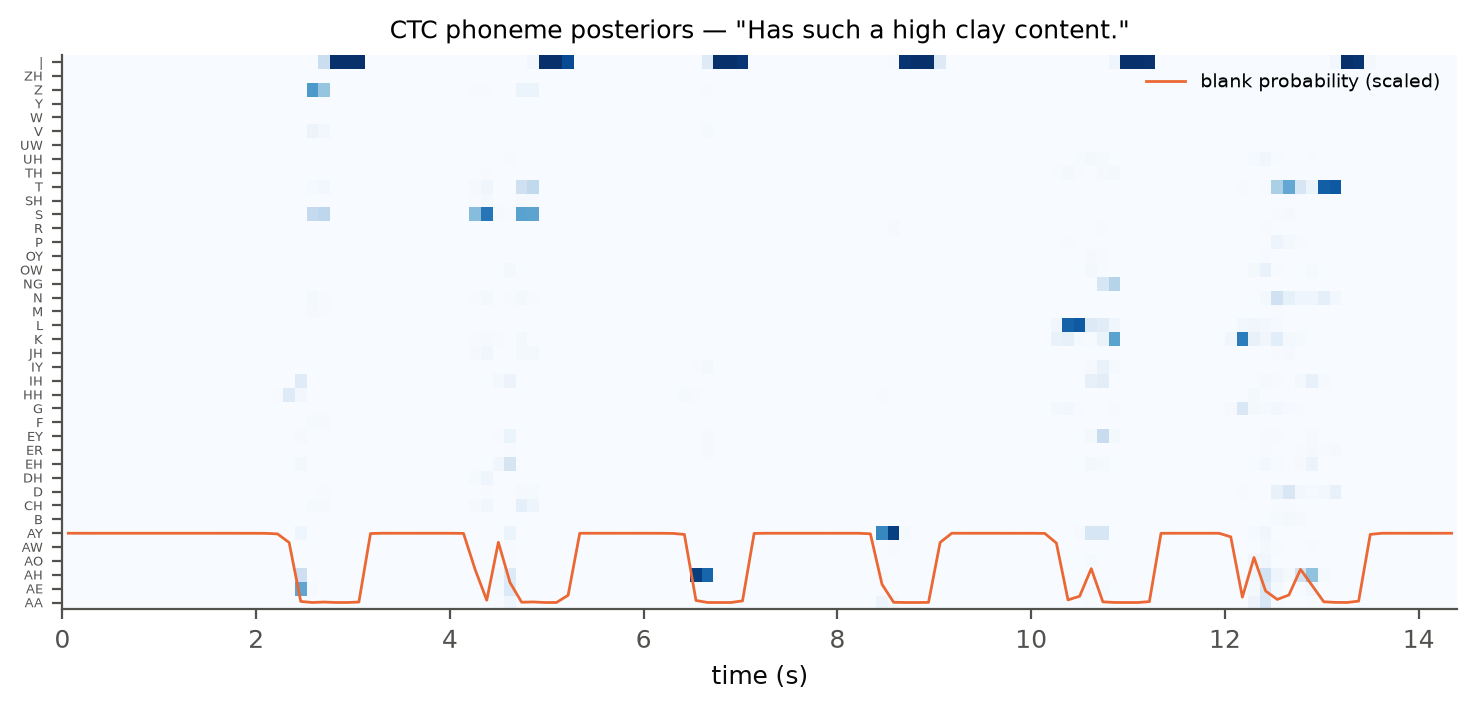
\includegraphics[width=\textwidth]{posteriors_example.png}
\caption{CTC phoneme posteriors of the causal Conformer (seed 0) on a held-out test sentence. Rows are the 39 phonemes plus the word boundary ``$|$''. The orange trace is the blank probability (scaled). The decoder emits sparse, peaky phoneme spikes separated by long blank stretches, typical of CTC. The beam search and LM turn these spikes into words.}
\label{fig:posteriors}
\end{figure*}

\subsection{Problem setup}
A trial gives features $\mathbf{x}_{1:T}\in\mathbb{R}^{T\times 512}$ recorded on day $d$, and a label sequence $\mathbf{y}=(y_1,\dots,y_L)$ over $\mathcal{V}=\{39\text{ phonemes},|\}$. A neural decoder $f_\theta$ outputs frame-level posteriors $p_\theta(k\mid\mathbf{x},t)$ over $\mathcal{V}\cup\{\varnothing\}$ (41 classes) at a reduced frame rate $T'$. Training minimizes the CTC loss
\begin{equation}
\mathcal{L}_{\text{CTC}}=-\frac{1}{L}\log\!\!\sum_{\pi\in\mathcal{B}^{-1}(\mathbf{y})}\prod_{t=1}^{T'}p_\theta(\pi_t\mid\mathbf{x},t),
\end{equation}
where $\mathcal{B}$ collapses repeats and then removes blanks.

\subsection{Shared front end}
\textbf{Day-specific input layers.} Each recording day $d$ has its own affine map, initialized to the identity, followed by a softsign:
$\tilde{\mathbf{x}}_t=\operatorname{softsign}(\mathbf{W}_d\mathbf{x}_t+\mathbf{b}_d)$, with $\mathbf{W}_d\in\mathbb{R}^{512\times512}$ and no weight decay on $\mathbf{W}_d,\mathbf{b}_d$. The ablation \emph{no day layers} shares a single $(\mathbf{W},\mathbf{b})$ across all days.
\textbf{Smoothing and patching.} Features are smoothed with a Gaussian kernel ($\sigma=40$\,ms, matching the published 2 bins of 20\,ms). Windows of $P$ consecutive bins are then concatenated with stride $S$ (``patching''), which sets the output frame rate.
On CPU we average every three consecutive 20\,ms bins into one 60\,ms bin and use $P{=}5$, $S{=}2$: 300\,ms windows every 120\,ms, against 280\,ms every 80\,ms in the published configuration. T15 speaks at about 32 words per minute, and our trials average 1.5 label tokens per second. At 120\,ms per frame that is about 5.5 frames per label, which leaves room for CTC blanks.

\subsection{Baseline: GRU--CTC}
The patched sequence feeds a unidirectional GRU (2 layers, 256 units; published: 5$\times$768) with dropout 0.4 and a linear read-out to 41 classes. GRU input-to-hidden weights use Xavier initialization and hidden-to-hidden weights use orthogonal initialization, as in the released code.
\textbf{Published augmentation} adds white noise ($\sigma{=}1.0$) and a per-trial, per-feature constant offset ($\sigma{=}0.2$), and randomly cuts up to one leading bin.

\subsection{New augmentations: time masking and electrode dropout}
Chronic arrays lose channels over months, and attempted speech is interrupted by pauses and breaths. We add two augmentations, both inspired by SpecAugment \citep{park2019specaugment}.
\emph{Time masking} zeroes up to two spans of up to 480\,ms each.
\emph{Electrode dropout} zeroes \emph{both} features of each electrode independently with probability $q=0.1$, for the whole trial. This simulates an electrode that has failed or gone silent, rather than i.i.d.\ feature noise.
Section~\ref{sec:robust} also uses the same operation as a test-time stressor.

\subsection{Proposed encoder: causal Conformer with self-conditioned CTC}
After the day layers, a per-bin linear bottleneck (512$\to$128) and a patch embedding (Linear+LayerNorm) produce $d{=}144$-dimensional frames. Four Conformer blocks follow \citep{gulati2020conformer}, each a macaron feed-forward $\to$ multi-head self-attention $\to$ convolution module $\to$ feed-forward, with a final LayerNorm. For streaming, attention is causally masked and the depthwise convolution (kernel 15) is left-padded. We use LayerNorm rather than BatchNorm inside the convolution module, so that inference does not depend on batch statistics.
We use no absolute positional encoding: causal masking and the convolutions carry order information. In pilot runs, an unscaled sinusoidal encoding swamped the small patch embeddings.
After block 2 we compute an \emph{intermediate CTC} loss with the shared output head \citep{lee2021intermediate}. Its posteriors are projected back into the residual stream, $\mathbf{h}\leftarrow\mathbf{h}+\mathbf{W}_c\,\mathrm{softmax}(\cdot)$, which is \emph{self-conditioned CTC} \citep{nozaki2021selfcond}. The total loss is $0.7\,\mathcal{L}_{\text{CTC}}+0.3\,\mathcal{L}_{\text{CTC}}^{\text{inter}}$.
A unit test checks causality: perturbing inputs after time $t$ leaves all outputs whose receptive field ends before $t$ unchanged, apart from the 60\,ms half-width of the smoothing kernel.

\subsection{Stabilised CTC training}
\label{sec:stable}
In the previous round of this study, one of two GRU seeds stalled in both GRU configurations and the Conformer spent about 150 steps emitting only blanks. Per-step traces (loss, pre-clip gradient norm and the fraction of frames whose arg\,max is blank; \S\ref{sec:stability}) showed that the stalled seed did \emph{not} suffer exploding gradients: after step 20 its gradient norm stayed near 1, so the clipping threshold of 10 was never reached. Instead, its first $\sim$20 steps were spent learning to emit blanks from a uniform initial posterior (initial loss $\approx$16, gradient norms up to 13 during warm-up), after which it sat on the ``blank plus frequent phonemes'' plateau that CTC models are known to pass through \citep{zeyer2021peaky}. We changed five things, all standard:
(i)~\textbf{blank-logit initialisation}: the read-out bias of the blank starts at $b{=}4$, so $p(\varnothing)=e^{b}/(e^{b}+40)=0.58$, close to the frame-level blank rate of a trained model, and the first updates go to the label logits;
(ii)~\textbf{input re-standardisation}: averaging three z-scored 20\,ms bins shrinks the feature s.d.\ to 0.63, so the published white-noise augmentation ($\sigma{=}1$, set for unit-variance inputs) had a 1.6$\times$ lower signal-to-noise ratio than intended; we rescale the binned features by one global constant (1/s.d.\ of the training features);
(iii)~\textbf{a short-utterance curriculum} for the first 100 steps (the shorter half of the training sentences), in the spirit of SortaGrad \citep{amodei2016deepspeech2};
(iv)~\textbf{a longer linear warm-up} (100 steps instead of 50) before the cosine decay \citep{loshchilov2017sgdr}; and
(v)~\textbf{gradient-norm clipping at 1} instead of 10 \citep{pascanu2013difficulty}, so that the rare large steps are bounded.
The Conformer keeps its intermediate, self-conditioned CTC loss, which also acts as an auxiliary signal for the lower blocks.

\subsection{Ensembling}
Following the Brain-to-Text~'24 lessons, we ensemble models of the same architecture trained with different seeds by averaging their per-frame posteriors, $\bar p(k\mid t)=\tfrac1M\sum_m p_{\theta_m}(k\mid t)$, and then decode $\bar p$.

\subsection{Phoneme-to-word decoding}
\textbf{Lexicon and LM.} The vocabulary is every word with a CMUdict pronunciation \citep{cmudict} that occurs at least twice in the LM corpus or appears in a training cue sentence: \LMVocab{} words, with \LMOOV\% out-of-vocabulary tokens on the evaluation sentences.
The corpus is OpenWebText-10k \citep{gokaslan2019openwebtext}, DailyDialog \citep{li2017dailydialog} and the cue sentences of the training trials, \LMWords\,M words in total. Any corpus sentence that matches a dev or test sentence after normalization is removed (\LMRemoved{} sentences).
We fit an interpolated Kneser--Ney trigram \citep{kneser1995improved,chen1999empirical} with discount $D{=}0.75$ (\LMTrigrams\,M trigrams). It is stored as sorted 64-bit keys and queried by binary search.

\textbf{Beam search.} Hypotheses walk a phoneme trie of the vocabulary under the CTC prefix recursion \citep{hannun2014firstpass}. When the decoder emits ``$|$'' at a trie node where one or more words end, the hypothesis commits each such word (homophones branch). Each committed word $w$ adds
\begin{equation}
\alpha\log P_{\text{KN}}(w\mid w_{-2},w_{-1})+\beta
\end{equation}
to the hypothesis score. A hypothesis that ends inside a word is completed or dropped, and the score for the end-of-sentence token is then added. We use beam 32. Frames with blank probability above 0.999 are skipped, and tokens with log-probability below $-8$ are pruned.
\emph{No-LM} decoding uses the same lexicon-constrained search with $\alpha{=}0$.

\textbf{LLM rescoring.} The 10-best list is rescored with
\begin{equation}
s=\log p_{\text{CTC}}+\alpha\log P_{\text{KN}}+\beta|w|+\gamma\log P_{\text{GPT-2}},
\end{equation}
where GPT-2 small (124M parameters; \citealp{radford2019gpt2}) stands in for the 6.7B-parameter OPT used clinically.
\textbf{Tuning on dev only.} All decoder settings are chosen on the 215 dev sentences (held-out trials of the training sessions, disjoint from the 426 test sentences), separately for each system, and the test set is then decoded once. The lexicon-only word bonus is searched first; $(\alpha,\beta)$ by two rounds of coordinate descent; then the beam width (8--64, ceiling 128); finally $\gamma$ jointly with a re-tuned word bonus on the dev 10-best lists. Every one-dimensional search starts from a grid and, whenever the optimum falls on an edge, extends the grid past that edge (multiplicatively for $\alpha$, $\gamma$ and the beam, additively for the bonuses) until the optimum is interior or a hard bound is reached ($\gamma\ge0$, beam $\le128$).

\subsection{Unsupervised adaptation to a new day}
\label{sec:tta}
For a new session we change only that day's input layer $(\mathbf{W}_d,\mathbf{b}_d)$, initialised from the most recent training day's layer, and use only \emph{unlabelled} neural data from the new day (its \texttt{train} split; never the test sentences).
\textbf{Feature-statistics matching} maps the new day's features onto the statistics of the most recent training day by an affine map $\mathbf{x}\mapsto\mathbf{x}\mathbf{A}+\mathbf{c}$ and folds it into the copied layer ($\mathbf{W}_d\leftarrow\mathbf{A}\mathbf{W}_{d-1}$, $\mathbf{b}_d\leftarrow\mathbf{c}\mathbf{W}_{d-1}+\mathbf{b}_{d-1}$). We use either per-feature mean/s.d.\ matching or CORAL \citep{sun2016coral}, $\mathbf{A}=\mathbf{C}_{\text{new}}^{-1/2}\mathbf{C}_{\text{ref}}^{1/2}$, with 10\% shrinkage of each covariance toward its diagonal.
\textbf{Self-training} \citep{kahn2020selftraining}, close in spirit to the LM-corrected self-recalibration of \citet{fan2023plug}: the unlabelled sentences are decoded with the lexicon + trigram beam search, the decoded words are turned back into phoneme targets with the pronunciation lexicon, and the half of the sentences whose greedy phoneme string agrees least with that pseudo-label (1\,$-$\,PER between the two) is discarded. The day layer is then fine-tuned with CTC on the rest for 40 steps, exactly as in supervised calibration, and the procedure is repeated for two rounds. We also run self-training starting from the CORAL-initialised layer.

\section{Experimental setup}
\label{sec:setup}

\paragraph{Data.} We use the Brain-to-Text~'25 release of \citet{card2024accurate} \citep{card2025dryad}. Dryad's API now requires a bearer token for downloads, so we stream the per-session HDF5 files from a public Hugging Face mirror of the unzipped release. Each file is converted to compressed float16 (48\% of the HDF5 size) and the HDF5 is deleted, which keeps the data under a 3\,GB disk budget.
We use \textbf{10 training sessions} spread over August--December 2023: 2{,}140 sentences in the released \texttt{train} split, of which 10\% per session are held out as a \emph{dev} set (215) for checkpoint selection and LM tuning. The \textbf{test set} is the released \texttt{val} split of the same sessions (426 sentences). The competition's \texttt{test} split has no labels.
A later session, \textbf{2024-03-15}, recorded 77 days after the last training session, never enters base training. It serves as the ``new day'' for calibration: 239 calibration sentences and 48 test sentences.
Trials average 18.3\,s (916 bins of 20\,ms) and 27 label tokens. The cue sentences come from Switchboard, OpenWebText, Harvard sentences, a frequent-word corpus, a 50-word corpus and random word sequences (see the block metadata in the released code). Our test set has \CorpusNSwitchboard{} Switchboard, \CorpusNFreqWords{} frequent-word, \CorpusNOpenwebtext{} OpenWebText, \CorpusNHarvard{} Harvard and \CorpusNRandom{} random-word sentences. No test sentence occurs in the training split.

\paragraph{Training.} We use AdamW (learning rate $2\times10^{-3}$, weight decay $10^{-2}$ excluding the day layers), batch 32, length-bucketed batches, 480 steps with 50 warm-up steps and cosine decay to 2\% (Conformer: 100 warm-up steps), and gradient clipping at 10. Dev greedy PER is evaluated every 50 steps and the best checkpoint is kept. On a shared 8-core Intel Mac with two threads per job, one run took 38--76 minutes depending on machine load. One run (GRU + new aug., seed 1) hit the 75-minute safety limit at step 466 of 480, when the learning rate had already decayed to about 2\% of its peak. The published schedule is 120{,}000 steps of batch 64, about 500$\times$ more samples.
The GRUs use two seeds (0, 1). The Conformer has one seed: its second seed, along with a third GRU seed, a no-day-layer and a no-augmentation ablation, and a trained bidirectional GRU, was stopped or dropped because the shared machine became oversubscribed (load average above 100). These runs are listed in \texttt{gpu.yaml}.

\paragraph{Systems.}
\begin{itemize}\itemsep0pt
\item \textbf{GRU baseline}: the published recipe, scaled down.
\item \textbf{GRU + new aug.}: adds time masking and electrode dropout.
\item \textbf{Causal Conformer}: \S\ref{sec:method}, with the new augmentations.
\item \textbf{Bidirectional GRU}: a non-causal reference, used for latency only (timed untrained).
\item \textbf{Day layers}: analyzed by swapping layers at test time (\S\ref{sec:results}).
\end{itemize}

\paragraph{Metrics.} PER and WER are corpus-level: total Levenshtein edits divided by total reference tokens, after lower-casing and removing punctuation. PER includes the word-boundary token, as in the released evaluation code. 95\% confidence intervals come from a bootstrap over sentences (2{,}000 resamples; \citealp{bisani2004bootstrap}). Systems are compared with a paired bootstrap over the same sentences (10{,}000 resamples; \citealp{koehn2004significance}); for a comparison of recipes we first average each sentence's edit count over the three seeds.

\section{Results}
\label{sec:results}

\begin{table*}[t]
\centering
\caption{Test-set results on 426 held-out sentences from the 10 training sessions. PER is from greedy CTC decoding. WER is from lexicon-constrained beam search without an LM, with the Kneser--Ney trigram, and after GPT-2 rescoring of the 10-best list. Multi-seed rows are mean\,$\pm$\,s.d.\ over seeds. ``Ensemble'' averages per-frame posteriors over the seeds. GPT-2 rescoring was run only on the best single models; $^\dagger$\,seed 0 only. The Conformer has a single seed (its second seed was stopped for lack of CPU time).}
\label{tab:main}
\begin{tabular}{lcccc}
\toprule
Model & PER & \multicolumn{3}{c}{WER} \\ \cmidrule(lr){2-2}\cmidrule(lr){3-5}
 & greedy & no LM & 3-gram & +GPT-2 \\
\midrule
GRU baseline (published recipe) (2 seeds) & 60.2\,$\pm$\,17.9 & 92.8\,$\pm$\,6.1 & 81.0\,$\pm$\,20.5 & 66.5$^\dagger$ \\
\quad ensemble of 2 & 75.3 & 95.7 & 87.2 & -- \\
GRU + time mask + electrode dropout (2 seeds) & 59.7\,$\pm$\,14.8 & 92.1\,$\pm$\,5.8 & 81.1\,$\pm$\,16.4 & -- \\
\quad ensemble of 2 & 75.7 & 95.3 & 85.9 & -- \\
Causal Conformer + SC-CTC (1 seed) & 38.8 & 83.2 & 52.1 & 51.7 \\
\bottomrule
\end{tabular}
\end{table*}

\begin{figure*}[t]
\centering
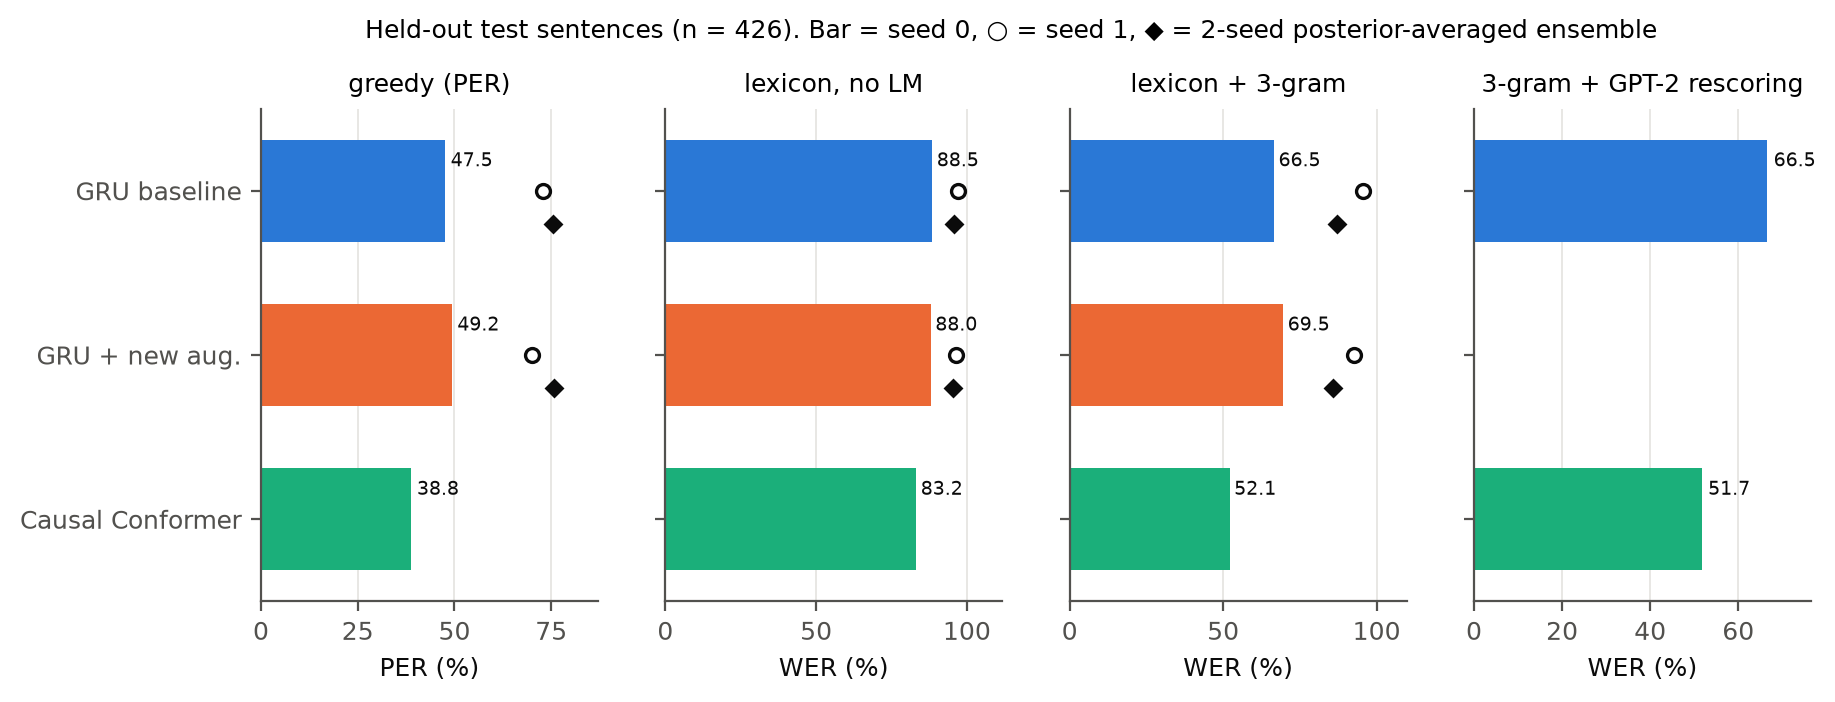
\includegraphics[width=\textwidth]{main_results.png}
\caption{Error rates per model and decoding stage (Table~\ref{tab:main}). Bars show seed~0, open circles seed~1, and diamonds the 2-seed posterior-averaged ensemble. GRU seed~1 stalled in both configurations, and averaging it into an ensemble degrades the converged seed.}
\label{fig:main}
\end{figure*}

\subsection{Neural decoders}
Table~\ref{tab:main} and Fig.~\ref{fig:main} give the main comparison.
The \textbf{causal Conformer} reaches \ConfPER\% PER and \ConfWERng\% WER with the trigram. The best GRU seed reaches \BaseSZeroPER\% PER and \BaseSZeroWERng\% WER (baseline, seed 0).
Its training curve (Fig.~\ref{fig:curves}) has a distinctive shape. For roughly the first 150 steps the Conformer predicts only blanks (dev PER 100\%): the CTC ``blank plateau''. It then improves faster than any GRU and ends below them. Two changes were needed to get there: removing the absolute positional encoding, and using a longer warm-up.
This matches the Brain-to-Text~'24 experience \citep{willett2024b2t}: attention-based encoders are harder to optimize on this data, but they are not intrinsically worse. A practical consequence is that a short pilot run can wrongly rule out a Conformer.

The \textbf{GRU recipe was seed-sensitive} at this budget. With seed~0, both GRU variants train normally (\BaseSZeroPER\% and \AugSZeroPER\% test PER). With seed~1, both stall (\BaseSOnePER\% and \AugSOnePER\%) (Fig.~\ref{fig:curves}, dashed). The mean\,$\pm$\,s.d.\ in Table~\ref{tab:main} reflects this bimodality rather than Gaussian noise. Averaging the posteriors of a converged seed with those of a stalled one is \emph{worse than either member}: \BaseEnsPER\% PER for the baseline ensemble and \AugEnsPER\% for the augmented one (Table~\ref{tab:ablation}). The stalled model's diffuse posteriors corrupt the confident ones. A production pipeline should gate ensemble members on dev PER.

\begin{figure}[t]
\centering
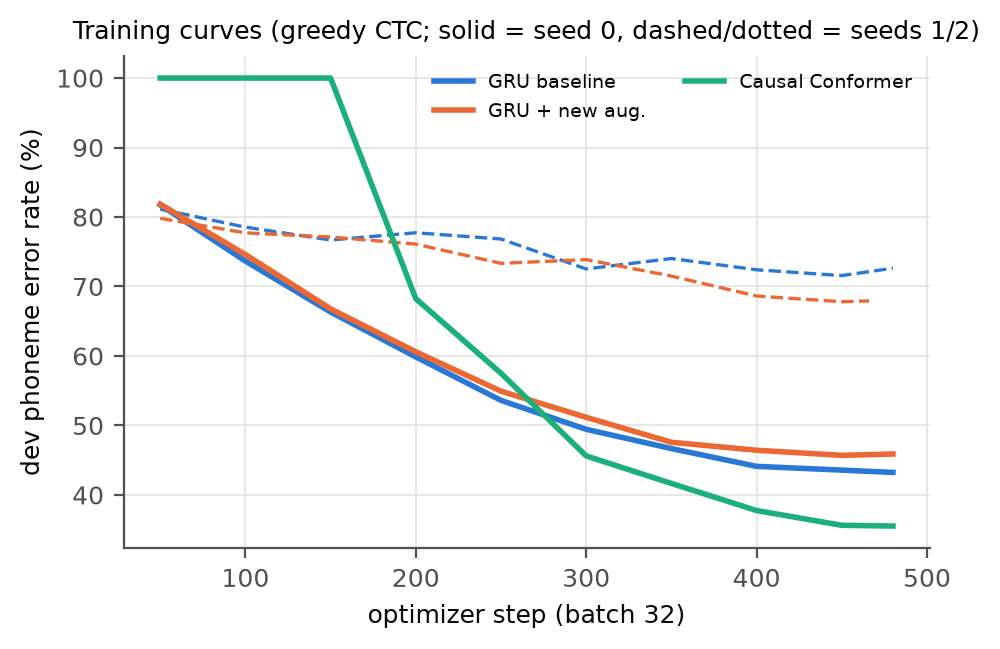
\includegraphics[width=\columnwidth]{training_curves.png}
\caption{Dev PER during training. The Conformer stays on the CTC blank plateau for about 150 steps, then overtakes the GRUs. GRU seed~1 (dashed) stalls for both augmentation settings.}
\label{fig:curves}
\end{figure}

\subsection{Augmentation and day-specific layers}
Table~\ref{tab:ablation} separates the components. \textbf{Time masking and electrode dropout} did \emph{not} improve clean test accuracy at this budget. With seed 0, PER is \AugSZeroPER\% against \BaseSZeroPER\% without them, a difference within the seed noise we observe. This is expected for an under-trained model that is not yet overfitting: regularization pays off when the model is data-limited rather than optimization-limited.
A modest benefit appears under electrode loss (\S\ref{sec:robust}).

\textbf{Day-specific input layers} matter. We evaluated the trained models with the \emph{wrong} day's layer, without retraining. For the GRU, using the previous session's layer raises PER from \SwapAugOwn\% to \SwapAugPrev\%; using the most distant session's layer (up to 4.5 months away) raises it to \SwapAugFar\%; replacing the layer by the identity gives \SwapAugIdent\%.
For the Conformer the corresponding numbers are \SwapConfOwn\%, \SwapConfPrev\%, \SwapConfFar\% and \SwapConfIdent\%. The penalty grows with the time between sessions, as expected from drifting recordings. Even the adjacent session's layer costs 3--6 points, which is why a new day needs calibration (\S\ref{sec:calib}). Interestingly, for the Conformer a distant day's layer is \emph{worse} than no day layer at all.
(We had planned a train-time ablation without day layers, but it did not fit the CPU budget; it is included in \texttt{gpu.yaml}.)

\begin{table}[t]
\centering
\caption{Component analysis. Augmentation: test PER/WER for seeds 0/1. Day layer: test PER when every session is decoded through a different input layer (no retraining), shown as GRU + new aug.\ / Conformer.}
\label{tab:ablation}
\resizebox{\columnwidth}{!}{\begin{tabular}{lcc}
\toprule
Configuration & PER & WER (3-gram) \\
\midrule
\multicolumn{3}{l}{\emph{Augmentation (GRU, per seed: s0 / s1)}} \\
\quad published (noise, offset, cut) & 47.5 / 72.8 & 66.5 / 95.5 \\
\quad + time mask + electrode dropout & 49.2 / 70.1 & 69.5 / 92.7 \\
\multicolumn{3}{l}{\emph{Ensembling (posterior average of s0+s1)}} \\
\quad GRU baseline & 75.3 & 87.2 \\
\quad GRU + new aug. & 75.7 & 85.9 \\
\multicolumn{3}{l}{\emph{Day-specific input layer at test time (PER only)}} \\
\quad own day & 49.2 / 38.8 & -- \\
\quad previous session's layer & 52.1 / 44.7 & -- \\
\quad most distant session's layer & 56.4 / 53.0 & -- \\
\quad identity (no day layer) & 58.1 / 48.5 & -- \\
\quad\footnotesize (GRU + new aug. / Conformer) & & \\
\bottomrule
\end{tabular}}
\end{table}

\subsection{Language-model stack}
\label{sec:lmres}
Table~\ref{tab:lm} shows where the word errors are removed.
Lexicon-constrained decoding without an LM performs poorly: \ConfWERlex\% WER for the Conformer, even though its PER is \ConfPER\%. A PER near 40\% leaves most words with at least one wrong phoneme, and the lexicon alone cannot repair them.
The trigram removes more than a third of the word errors, bringing the Conformer to \ConfWERng\% (bootstrap 95\% CI \ConfNGlo--\ConfNGhi\%).
GPT-2 rescoring of the 10-best list helps only marginally (\ConfWERllm\%, with $\gamma=0.75$ chosen on dev). For the GRU, dev tuning selected $\gamma=0$, so rescoring changes nothing.
The \emph{oracle} over the 10-best list is \ConfOracle\% for the Conformer and \BaseOracle\% for the GRU. With error rates this high, the correct sentence is rarely in the list at all, so no rescorer can help much. Clinical systems rescore from a far stronger starting point.
For this regime, the order of priorities is a better neural decoder first and a better LM second.
The LM's contribution also depends on the material (Fig.~\ref{fig:corpus}). Conversational Switchboard sentences reach \CorpusSwitchboard\% WER, but random word sequences, where the LM can only hurt, reach \CorpusRandom\%.

\begin{figure}[t]
\centering
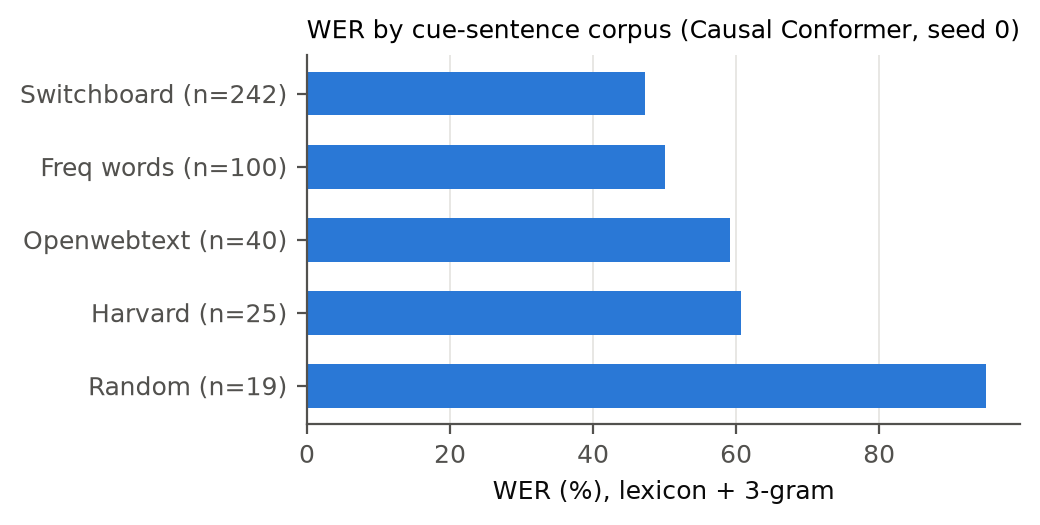
\includegraphics[width=\columnwidth]{wer_by_corpus.png}
\caption{Conformer (seed 0) test WER with the trigram, by cue-sentence corpus.}
\label{fig:corpus}
\end{figure}

\begin{table}[t]
\centering
\caption{WER (\%) at each decoding stage. ``Oracle@10'' is the lowest WER reachable by choosing within the trigram decoder's 10-best list.}
\label{tab:lm}
\resizebox{\columnwidth}{!}{\begin{tabular}{lccccc}
\toprule
System & greedy PER & no LM & 3-gram & +GPT-2 & oracle@10 \\
\midrule
Conformer (s0) & 38.8 & 83.2 & 52.1 & 51.7 & 48.2 \\
GRU baseline (s0) & 47.5 & 88.5 & 66.5 & 66.5 & 63.1 \\
GRU baseline ens. & 75.3 & 95.7 & 87.2 & -- & -- \\
GRU + new aug. ens. & 75.7 & 95.3 & 85.9 & -- & -- \\
\bottomrule
\end{tabular}}
\end{table}

\subsection{Calibration to a new day}
\label{sec:calib}
Figure~\ref{fig:calib} shows what happens on session 2024-03-15, 77 days after the last training session, using the GRU + new aug.\ (s0) model.
Without any new data, reusing the most recent day's layer gives \CalReusePER\% PER and \CalReuseWER\% WER. The same model gets \AugSZeroPER\% PER on in-distribution sessions.
Fine-tuning \emph{only the new day's input layer} on 25 sentences, a few minutes of attempted speech, lowers WER to \CalDayTwentyFiveWER\%. With 200 sentences it reaches \CalDayTwoHundredWER\%.
Fine-tuning \emph{the whole network} on the same sentences is no better from 25 sentences on: \CalFullTwentyFiveWER\% at 25 sentences and \CalFullTwoHundredWER\% at 200. At 10 sentences the two are tied (\CalFullTenWER\% vs.\ \CalDayTenWER\%). It also changes every weight, which is a larger regulatory and safety surface for a medical device than retraining one input layer.
The test set for this day is small (48 sentences), so differences of 2--3 WER points are within noise (bands in Fig.~\ref{fig:calib}).

\begin{figure*}[t]
\centering
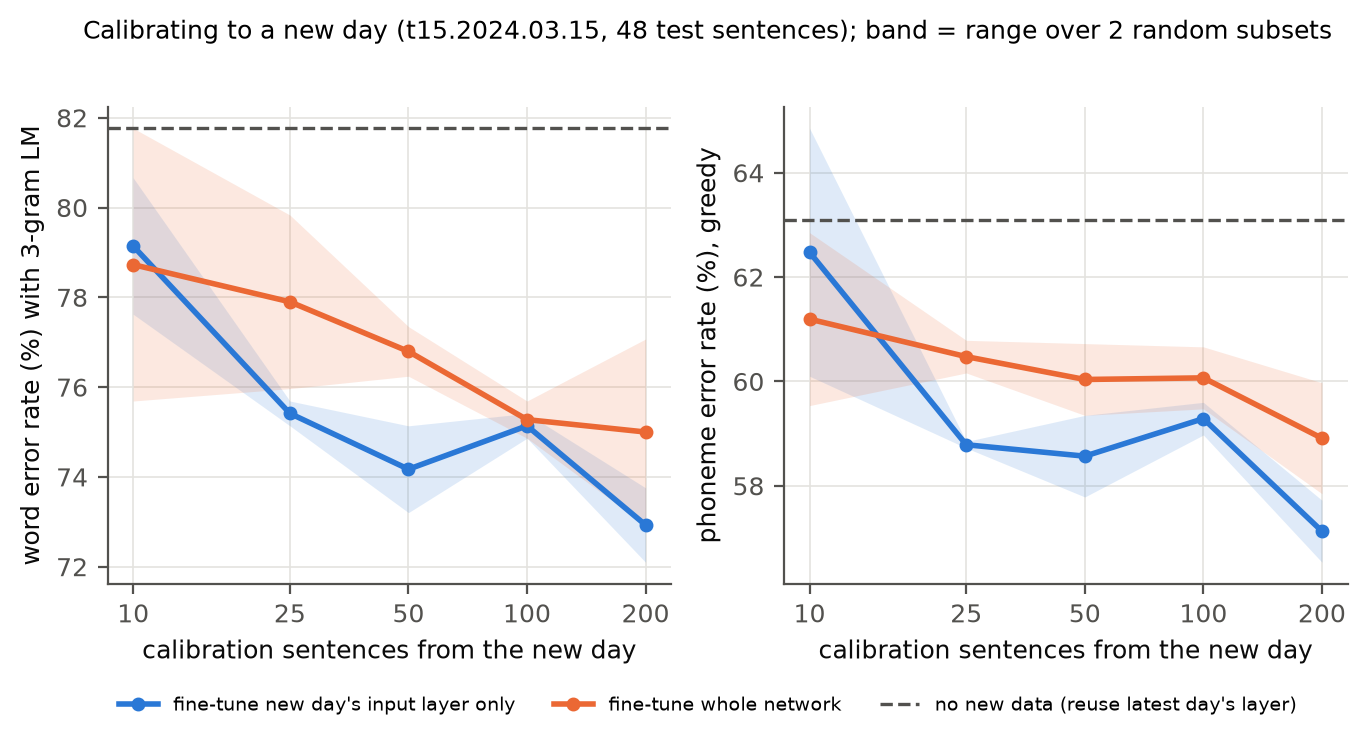
\includegraphics[width=\textwidth]{calibration.png}
\caption{Calibrating to a new day 77 days after training. Day-layer-only fine-tuning recovers most of the attainable improvement within 25 sentences. Full fine-tuning is no better. Bands show the range over two random subsets of calibration sentences.}
\label{fig:calib}
\end{figure*}

\subsection{Robustness to electrode loss}
\label{sec:robust}
Figure~\ref{fig:robust} silences a random fraction of electrodes (both features) at test time, without recalibration.
Silencing 10\% of electrodes costs about one PER point for every model: GRU baseline \RobBaseZero\% $\to$ \RobBaseTen\%, GRU + electrode dropout \RobAugZero\% $\to$ \RobAugTen\%, Conformer \RobConfZero\% $\to$ \RobConfTen\%.
At 50\% loss the GRUs reach \RobBaseFifty\% and \RobAugFifty\%. The model trained with electrode dropout started 1.7 points worse but degraded less, so the gap between the two GRUs has closed. The Conformer degrades the most in absolute terms (to \RobConfFifty\%) but stays the best model at every level of loss.
Decoding is therefore graceful under channel loss: the 512 features are highly redundant for this task. Electrode dropout buys a modest reduction in the slope. Only one random electrode subset was drawn per fraction, so small differences are not significant.

\begin{figure}[t]
\centering
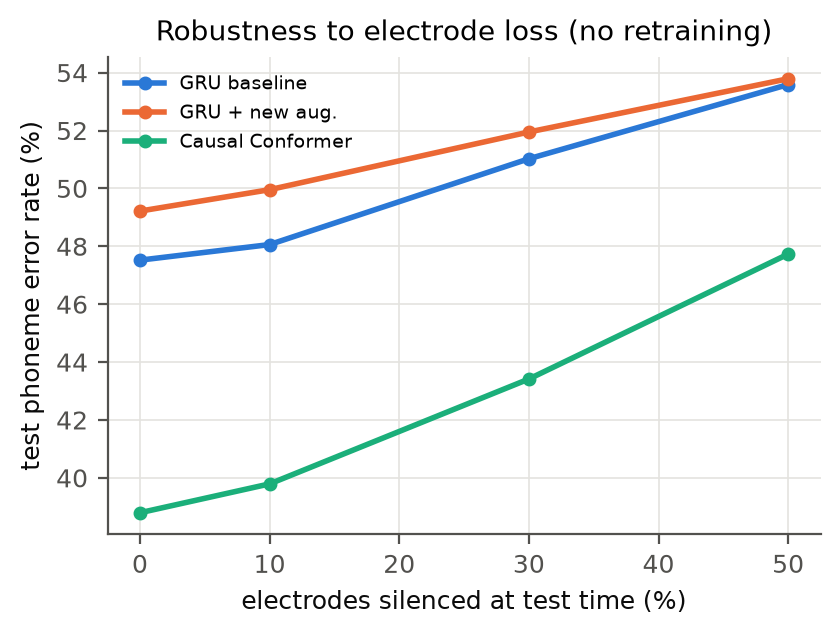
\includegraphics[width=\columnwidth]{robustness.png}
\caption{Test PER when a random subset of electrodes is silenced (one random subset per fraction), with no retraining.}
\label{fig:robust}
\end{figure}

\subsection{Latency and compute}
Table~\ref{tab:latency} reports CPU costs, measured with 2 threads on a heavily shared machine (minimum over 7 repeats, to limit contention effects; absolute values still vary severalfold with load).
The causal GRU costs \LatAugFrame\,ms of compute per 120\,ms output frame when streamed step by step, which is dominated by per-step overhead in PyTorch. The causal Conformer's amortized cost is \LatConfFrame\,ms per frame with a key/value cache. Without a cache, recomputing a 64-frame (7.7\,s) window every frame costs \LatConfRecompute\,ms. That still fits within the 120\,ms frame budget on this CPU, but it wastes about 100$\times$ the cached compute, which matters for power on an implant-class processor.
Both causal models need only the 60\,ms half-width of the smoothing kernel as lookahead. A bidirectional decoder cannot emit anything until the sentence ends.
The language-model stages dominate the latency: \BeamMs\,ms per sentence for our pure-Python beam search and \GPTMs\,ms for GPT-2 rescoring. This argues for streaming word-level beam search (as in WFST decoders) with rescoring only at sentence end.

\begin{table}[t]
\centering
\caption{CPU compute (2 threads) on a median-length test sentence (17\,s). ``Per frame'' is the incremental cost of one 120\,ms output frame. The bidirectional GRU was timed untrained, which does not change its compute.}
\label{tab:latency}
\resizebox{\columnwidth}{!}{\begin{tabular}{lrrrr}
\toprule
Model & params & full fwd & per frame & lookahead \\
 & (M) & (ms) & (ms) & (ms) \\
\midrule
GRU + time mask + electrode dropout & 5.46 & 75 & 2.6 & 60 \\
Bidirectional GRU + new aug. & 8.42 & 161 & -- & sentence \\
Causal Conformer + SC-CTC & 4.99 & 46 & 0.3 & 60 \\
\bottomrule
\end{tabular}}
\end{table}

\section{Discussion: what this means for a speech product}
\label{sec:discussion}

\paragraph{Optimization robustness is part of the product.} One of the two GRU seeds stalled in both GRU configurations, and the Conformer sat on a blank plateau for about 150 steps. A decoder that is retrained or recalibrated in the field, with no expert watching it, needs automatic acceptance checks: dev PER thresholds, plateau detection with restarts, and gating of ensemble members. Average accuracy is not enough.

\paragraph{Calibrate the input layer, not the decoder.} From 25 calibration sentences upward, updating a single $512\times512$ day layer was at least as good as fine-tuning everything (the two were tied at 10). Its benefit had largely saturated at about 25 sentences. Day-layer calibration is cheap (40 gradient steps on one layer), easy to validate and easy to roll back. That makes it a natural ``start of day'' routine, with unsupervised continual recalibration \citep{fan2023plug} as the next step.

\paragraph{Design for drift and channel loss.} A mismatched day layer costs 3--14 PER points, depending on the time between sessions. Losing half the electrodes costs 5--9 points. Both effects are smaller than we expected, because of feature redundancy across the 256 electrodes. Augmentations that simulate deployment failure modes, such as electrode dropout, flatten the degradation slightly even when they do not improve clean accuracy. Telemetry on channel health, together with time since the last calibration, should trigger recalibration.

\paragraph{The LM can only fix what the decoder nearly got right.} The trigram removes more than a third of the word errors, but at PER around 40\% even the 10-best oracle stays near 48\% WER, and GPT-2 rescoring adds little. LLM-based correction pays off once the neural decoder is good, as in the clinical systems at 10--20\% PER. In our regime, the encoder (Conformer vs.\ GRU: $-$14 WER points) is the bigger lever.

\paragraph{Latency.} Causal neural decoders cost \LatConfFrame--\LatAugFrame\,ms of CPU per 120\,ms frame, well within real time. The current bottlenecks are the Python beam search and the LLM rescorer. Production systems should stream a compiled word-level search and confine LLM rescoring to sentence boundaries or run it asynchronously.

\section{Limitations}
\label{sec:limits}
\begin{itemize}\itemsep0pt
\item \textbf{Scale.} Each model sees about 15k training samples: 480 steps of batch 32, 1/500 of the published schedule. It is trained on 10 of 45 sessions, with a 2-layer, 256-unit GRU instead of 5$\times$768. Absolute error rates are therefore several times the clinical numbers and should not be compared with them. Relative conclusions may change at scale. In particular, the early-training advantage of the Conformer and the penalty from the new augmentations are both measured in a heavily under-trained regime.
\item \textbf{Seeds.} The GRUs have 2 seeds and the Conformer 1. Seed 1 stalled for both GRU variants. The Conformer's advantage (9 PER points over the best GRU seed) is large, but it rests on a single run and needs replication (\texttt{gpu.yaml} uses 3 seeds). The electrode-loss curves use one random subset per fraction.
\item \textbf{Compute contention.} Runs shared an oversubscribed CPU, so wall-clock timings vary by about 2$\times$. Step budgets are identical across runs, so the comparisons are fair in optimization steps but not in wall-clock time.
\item \textbf{LM.} Our trigram is trained on 5.7M words, orders of magnitude less text than the published 5-gram, and GPT-2 small is 54$\times$ smaller than OPT-6.7B. We include the training cue sentences in the LM corpus, as a deployed system that knows its prompt corpus would. Evaluation sentences are filtered out.
\item \textbf{One participant.} All data come from T15. Nothing here speaks to transfer across participants or to other array placements, such as Neuralink's thread-based electrodes.
\item \textbf{Calibration test set.} The new day has only 48 test sentences (about 360 words), so the calibration curve has wide uncertainty.
\item \textbf{Latency.} Measured on a contended laptop CPU in Python, not on implant-grade hardware. The Conformer's streaming cost assumes a key/value cache, which we did not implement.
\end{itemize}

\section{Broader impact and safety}
\label{sec:impact}
Speech BCIs can give back conversation to people who have lost it. A decoder that \emph{substitutes plausible words} is also a risk: a strong LM can turn a garbled neural signal into a fluent sentence the user never intended. In our results the LM removes more than a third of the word errors relative to lexicon-only decoding, which shows how much of the output the LM itself contributes. Product requirements should therefore include confidence display, easy correction and undo, and a ``not what I meant'' signal. As decoders improve, the 10-best oracle gap (\S\ref{sec:lmres}) suggests that a user-facing $n$-best selection interface could recover additional errors.
Motor-cortex decoding of \emph{inner} speech \citep{kunz2025inner} raises a privacy concern: decoders should be gated on intent, and posteriors and transcripts should stay on device. Finally, the public dataset comes from a single volunteer. Our filtering of evaluation sentences from the LM corpus and our use of only released, de-identified data follow the data-use terms.

\section{Reproducing at full scale}
\label{sec:repro}
Everything above is produced by \texttt{scripts/run\_cpu.sh} with \texttt{configs/cpu.yaml}. The script is resumable and caches each stage. \texttt{CONFIG=configs/smoke.yaml} runs the whole pipeline in about 15 minutes as an integration test.
\texttt{scripts/run\_gpu.sh} runs the same code with \texttt{configs/gpu.yaml} on a fresh Linux/CUDA machine. It creates a virtual environment from \texttt{requirements-gpu.txt}, downloads all 45 sessions (about 11\,GB as float16), and trains at the published scale: 20\,ms bins, 14-bin patches with stride 4, a 5$\times$768 GRU, an 8-layer 256-dimensional Conformer, 60k steps of batch 64, AMP, and three seeds per model. It then runs the same evaluation, calibration, robustness and latency studies. We expect the next gains to come from diphone targets \citep{li2024dcond}, a larger LM, an LLM rescorer of 1B+ parameters, and LLM-based ensemble merging \citep{willett2024b2t}.

\section{Conclusion}
We built an open, tested speech-neuroprosthesis pipeline that runs end to end on a laptop CPU, from public intracortical recordings to text. Under a 1/500 optimization budget, a causal Conformer with self-conditioned CTC beat the published GRU recipe on both PER and WER once it escaped an initial blank plateau. The pipeline also gave product-relevant answers. Calibrating only the day layer on about 25 sentences is a safe default for a new day. Decoding degrades gracefully as electrodes are lost. Optimization failures, not average accuracy, are the main reliability risk. And the LM stages, not the neural decoder, dominate latency.

\paragraph{Acknowledgements.} We thank the T15 participant and the BrainGate2 and UC Davis Neuroprosthetics Lab teams for releasing their data and code.



\bibliographystyle{abbrvnat}
\bibliography{refs}

\end{document}
